\subsection{Optika}

V~tejto kapitole si ukážeme prekvapivý súvis Fourierovej transformácie
s~fyzikálnym javom nazývaným interferencia svetla. Aby sme sa však
dopracovali k~tomuto výsledku, musíme najskôr prejsť sadou definícií a
viet.

% {{{ interferencia
\begin{definicia}
Interferenciou vĺn budeme nazývať fyzikálny fenomén, ktorý
nastáva, keď sa dve alebo viac vĺn putujúcich spoločným médiom
stretne.
\end{definicia}
% }}}

% {{{ superpozicia
\begin{veta}
Princípu superpozície (Huygensov princíp):
Nech $A(r,t)$ je amplitúda prvej vlny na mieste $r$ v~čase $t$.
Podobne, nech $B(r,t)$ je amplitúda druhej vlny.
Výsledkom interferencie vĺn A,B je vlna C, pre ktorú platí
 $C(r,t)=A(r,t)+B(r,t)$. 
\end{veta}

Princíp superpozície a interferencia vôbec sa vo
 fyzike používa na viacerých miestach a to najmä v~kvantovej fyzike.
Názornú ukážku skladania vĺn možno vidieť na obrázku
 \ref{fig:interferencia}.
% }}}

% {{{ obrazky k superpozicii

 \begin{figure}[htp]
 \centering
 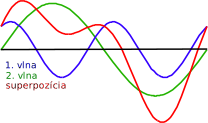
\includegraphics{obrazky/optika/interferencia_1}
 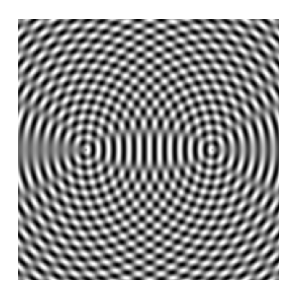
\includegraphics{obrazky/optika/interferencia_2}

 \caption{Interferencia 2 vĺn a) na priamke b) na ploche}
 \label{fig:interferencia}
 \end{figure}
% }}} 

Pre jednoduchosť budeme uvažovať interferenciu monochromatických vĺn.
Prax ukazuje, že zaujímavá vie byť aj všeobecná interferencia,
napríklad farebné sfarbenie povrchu bublín či olejových škvŕn. 
Táto téma je však nad rámec tejto publikácie.
\\

Majme zdroj (skalárneho) vlnenia v~3-rozmernom priestore.
Ak je poloha zdroja $\vect{a}$, amplitúda $A$, počiatočná fáza $\phi$ a vlnová dĺžka
$\lambda$, tak v~čase $t$ bude na mieste $\vect{r}$ výsledná amplitúda rovná

\begin{equation}
X(\vect{r},t)=A \cos \left(2 \pi \frac{|\vect{r}-\vect{a}| - t
c}{\lambda}+\phi \right)
\end{equation}

Podľa princípu superpozície pre $N$ zdrojov $1,\dots,N$ platí
\begin{equation}
X(\vect{r},t)=\sum_{i=1}^{N} A_i \cos \left(2 \pi
\frac{|\vect{r}-\vect{a_i}| - t c}{\lambda}+\phi_i \right)
\label{eq:interferencia}
\end{equation}

V ďalšom texte budeme využívať objekt zvaný "komplexná amplitúda".
Taktiež si ukážeme jeho aplikáciu pri riešení problému interferencie.

\begin{definicia}
Nech má vlna amplitúdu $A$ a fázu $\phi$.
Pod pojmom komplexná amplitúda budeme rozumieť komplexné číslo
$\mathcal{A}=A e^{i \phi}$.
\end{definicia}

\begin{poznamka}
 Komplexná amplitúda je akési prirodzené rozšírenie amplitúdy 
 o~fázu. Zvedavý čitateľ si určite kladie otázku k~čomu je dobrý iný
 zápis. Komplexná amplitúda je ale viac ako iný zápis, ako uvidíme
 neskôr, keď sa ukáže výhodné mať aj imaginárnu časť amplitúdy.
\end{poznamka}


\begin{lema}
Reálna časť komplexnej amplitúdy je amplitúda vlny v~danom bode.
\end{lema}
\begin{dokaz}
$\mathcal{A}=A e^{i \phi} = A (\cos \phi + i \sin \phi) =
A \cos \phi + i A \sin \phi$
\end{dokaz}

\begin{lema}
Interferencia z~rovnice \ref{eq:interferencia} sa pomocou
komplexnej amplitúdy dá popísať rovnicou
\begin{equation}
\mathcal{X}(\vect{r},t)=\sum_{i=1}^{N} 
A_i 
\exp \left[2 \pi i
\frac{|\vect{r}-\vect{a_i}| - t c}{\lambda}+ \phi_i i \right]
\end{equation}
resp.
\begin{equation}
\mathcal{X}(\vect{r},t)=\sum_{i=1}^{N} 
\mathcal{A}_i \exp \left[2 \pi i \frac{|\vect{r}-\vect{a_i}|
-tc}{\lambda}  \right]
\end{equation} 
\end{lema}

Túto rovnicu navyše ešte môžeme prepísať do spojitejšej verzie (budeme
uvažovať plošné zdroje vlnenia)
\begin{equation}
\mathcal{X}(\vect{r},t)=\int_S
 \mathcal{A} \exp \left[2 \pi i \frac{|\vect{r}-\vect{a}|
 -tc}{\lambda} \right] dS
\end{equation}

kde $\mathcal{A}, \phi$ závisia od plôšky $dS$ a $\mathcal{A}$
vyjadruje "plošnú hustotu komplexnej amplitúdy".

\begin{poznamka}
 Našim cieľom bude zhodnotiť energiu rýchlo kmitajúcej vlny.
 Čitateľ si môže všimnúť analógiu tohoto deja s elektrickou
 energiou. Keď máme jednosmerný obvod, energia ktorá sa spotrebúva
 napríklad na rezistore je časovo konštantná. Naproti tomu za
 prítomnosti striedavého napätia táto energia (za jednotku času) kolíše
 a v praxi nás zaujíma len jej stredná hodnota. To isté môžeme
 uvažovať aj u svetla, kedy nás nezaujíma energia (resp.
 pravdepodobnosť výskytu fotónov z kvantovej mechaniky) 
 na danom mieste v konkrétnom čase,
 ale jej stredná hodnota v čase, lebo to je veličina ktorú vieme merať.
\end{poznamka}


\begin{veta}
Energia ustredená cez čas pruslúchajúca vlne s~komplexnou amplitúdou 
$\mathcal{A}$ je $E \thickapprox |\mathcal{A}|^2$.
\label{veta:meanEnergy}
\end{veta}

\begin{poznamka}
 Viac o energii elektromagnetickej vlny sa dá dočítať 
 v~\cite[str. 90-92]{eldyn}, prípadne hľadajúc frázu "Poynting vector".
\end{poznamka}

Veta \ref{veta:meanEnergy} nám umožňuje jednoducho vymazať
$\exp\left(-2 \pi i \frac{tc}{\lambda}\right)$, nakoľko daný výraz má
jednotkovú komplexnú veľkosť a ovplyvňuje iba výslednú fázu.
V~duchu mazania premenných budeme pokračovať aj
naďalej a preto prehlásime $\phi=0$ (teda $\mathcal{A}=A$).
Fyzikálne toto decimovanie
ľahko ospravedlníme - väčšinou nás zaujíma interferencia
z~mriežky či otvorov, na ktoré svietime laserovým lúčom. Laserový
lúč je ale koherentný a preto môžeme uvažovať rovnakú fázu na celej
ploche. Stačí nám preto pokračovať s rovnicou

\begin{equation}
\mathcal{X}(\vect{r})=\int_S
 A \exp \left[2 \pi i \frac{|\vect{r}-\vect{a}|}{\lambda} \right] dS
\end{equation}

Ďalej budeme uvažovať, že plocha $S$ je malá a navyše nech je
blízko stredu súradicovej sústavy a nech leží v~rovine yz.
\footnote{Toto sú bežné predpoklady pri interferencii svetla}

Daný integrál si prepíšeme do formy

\begin{equation}
\mathcal{X}(\vect{r})=
 \exp \left[ 2 \pi i \frac{|\vect{r}|}{\lambda} \right]
\int_S A
 \exp \left[ 2 \pi i \frac{|\vect{r}-\vect{a}|-|\vect{r}|}{\lambda}
 \right] dS
 \label{eq:int42} 
\end{equation}
Teraz využijeme naše predpoklady o~tom, že $a \ll 1$
Rozvinieme 
$\displaystyle f(a)=|\vect{r}-\vect{a}|-|\vect{r}| =
\sqrt{ (\vect{r}-\vect{a})^2 } - r =
\sqrt{ \vect{r}^2 - 2 \vect{r}\vect{a} + \vect{a}^2 } -r$
do taylorovho radu v bode 0, a dostaneme
$f(a)=-\frac{\vect{r}.\vect{a}}{r} +O(a^2)$.

Rovnica \ref{eq:int42} prejde na
\begin{equation}
\mathcal{X}(\vect{r})=
 \exp \left[ 2 \pi i \frac{r}{\lambda} \right]
\int_S A
 \exp \left[- 2 \pi i \frac{\vect{r}.\vect{a}}{\lambda r} \right] dS
\end{equation}

Ak by nás nezaujímala interferencia svetla, ale napríklad mikrovlnného
žiarenia, bol by člen 
$\exp \left(2 \pi \frac{r}{\lambda} \right) $ dôležitý.


\todo{dorazenie, uz tam vidno fourierku po zlozkach}

Nech $\vect{a}=(x,y,0), \vect{r}=(u r \lambda, v r \lambda,z r \lambda)$ pričom
$u^2 + v^2 + z^2=\frac{1}{\lambda^2}$.
Potom $ \displaystyle
\mathcal{X}(u,v)=
\int \int A(x,y)
 \exp \left[- 2 \pi (xu+yv) \right] dx dy$.
V~týchto premenných dostávame teda $\mathcal{X}=\fourier[A]$.

\todo{toto je v podstate premietanie na gulu} \\
\todo{preratanie na plosne zobrazovanie} \\
\todo{mikrovlny verzus normalne vlny - dolezita faza} \\
\todo{inverzna transformacia - preco nejde? / v mikrovlnach vlastne
ide, ale je neuzitocna} \\
\todo{obrazky interferencie}
\todo{\cite[kap. 10]{holo} \cite{amsci} \cite{trester} }
